\documentclass[../diploma.tex]{subfiles}
 
\begin{document}

\subsection{Реализация модели}

Мы старались реализовать практическую часть так, чтобы она принесла максимальный вклад в сообщество и не затерялась в качестве приложения к исследовательской работе. Среди открытых реализаций не нашлось ни одной, котрая в полной мере реализовывала бы все заявленные архитектурные нюансы WaveNet. 
Поэтому было решено доработать архитектуру в виде ответвления от самого известного в сообществе решения.

Таким образом, реализацию можно разделить на две большие части: модификацию архитектуры сети и извлечение построение каскада признаков признаков. 
Также стоит удостоить внимания постановку экспериментов, но мы уделим им отдельный раздел \ref{sec:experiments}.
% Я там что-то реализовал причём сделал это так-то. Щас расскажу по пунктам.

Срез архитектуры сети до модификаций имеет структуру, изображенную на рисунке \ref{fig:arch_high}.

\begin{figure}[!htbp]
  \centering
  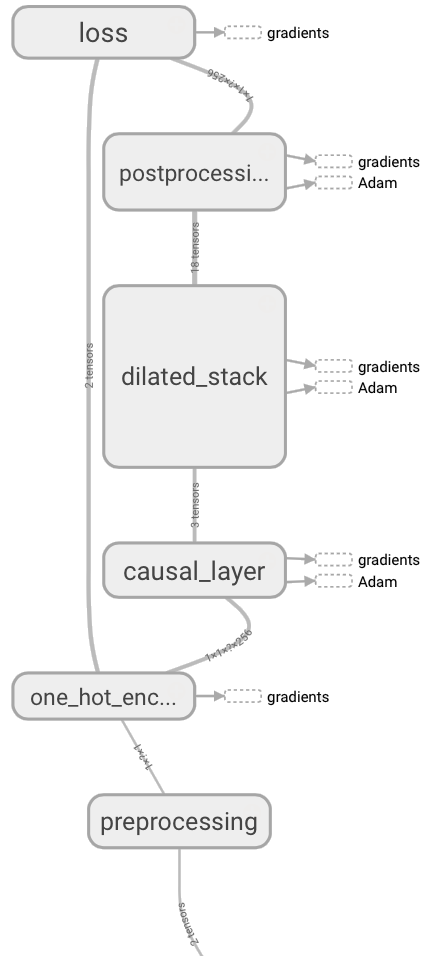
\includegraphics[scale=1.1]{img/network}
  \caption{Высокоуровневое описание архитектуры сети}
  \label{fig:arch_high}
\end{figure}


% Надо было запилить две фичи: локальные и глобальные условия. 
% Сначала надо понять, куда добавлять изменения, давай посмотрим на архитектуру и покажем, куда можно воткнуть условия.

% \begin{definition}
% Gate в контексте нейросетей это термин, мигрировавший из электрических сетей. Поскольку любые операции могут быть описаны в качестве графорвых примитивов, gate в самом широком смысле можно назвать операцию любой арности. Одним из простейших примеров gate является умножение.

% Ключевой gate в архитектуре называемый update gate находится на выходе из каждого пачки свёрточных слоёв.

% сделай, чтобы не съезжала

Реализация WaveNet, описываемая в этом разделе, реализована на языке Python на фреймворка для численных графовых вычислений c открытым исходным кодом Tensorflow. На момент написания статьи Tensorflow удерживает позицию одного из самого популярного фреймворков для проектирования и промышленной разработки нейронных архитектур.
По ходу раздела мы будем переключатся между абстрактным описанием WaveNet и обозначениями в вычислительном графе конкретной реализации, однако я постараюсь поддерживать единообразные наименования, чтобы не вызывать у читателя лишнего дискомфорта.

\begin{figure}[!htbp]
  \centering
  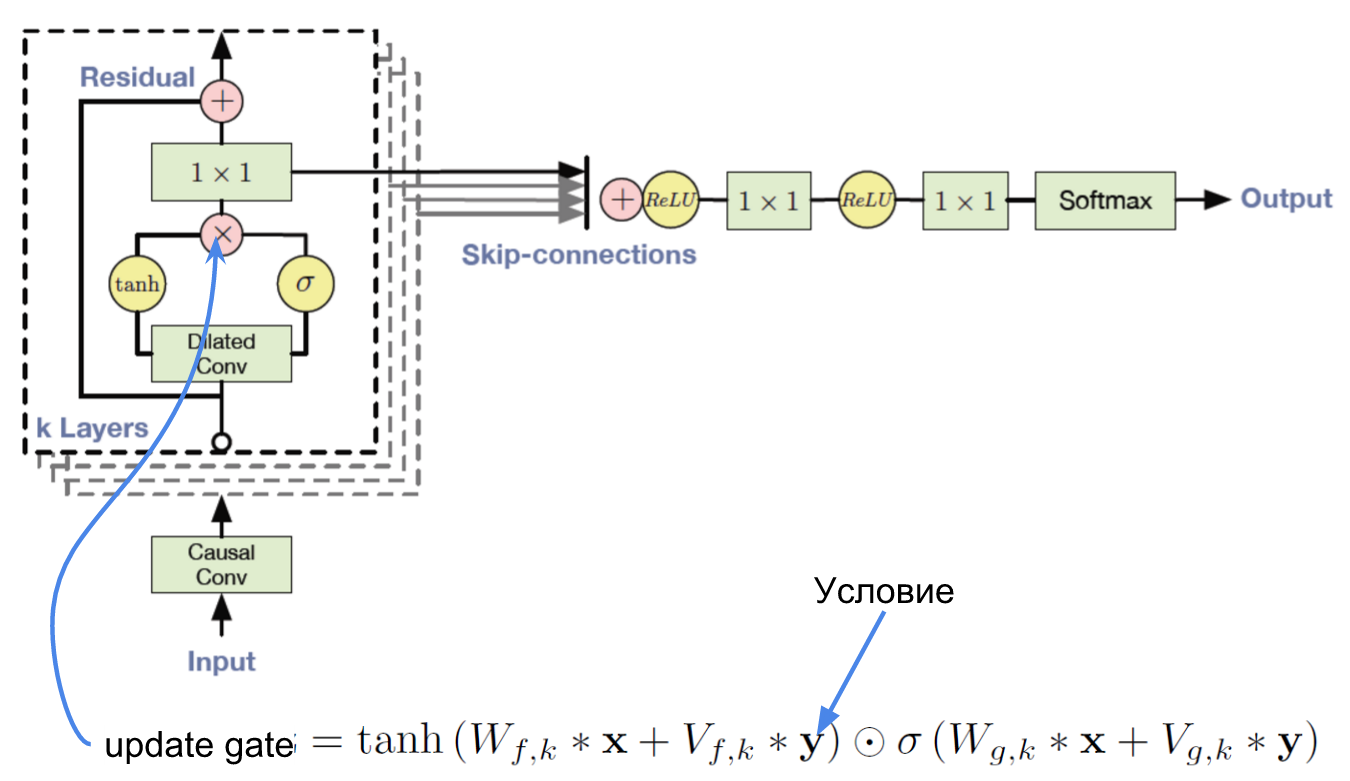
\includegraphics[scale=0.35]{img/wavenet_arrow}
  \caption{Gate, отвечающий за условия}
  \label{fig:wavenet_arrow}
\end{figure}

На рисунке \ref{fig:wavenet_arrow} заметно, что в архитектуре дублируются $k$ раз одинковые конструкции которые мы отныне будем называть \textbf{dilated stack}. Из каждого dilated stack выходит skip соединение на активационный gate и residual соединение в самого себя. Основной частью dilated stack является стэк свёрточных слоёв единообразной конфигурации, задаваемой в гиперпараметрах сети.

Как мы уже знаем, дополнительные условия передаваемы WaveNet должны быть переданы в update gate \ref{fig:wavenet_arrow}. А так как такой gate есть в каждом dilated stack, мы на самом деле должны продублировать эти условие тоже $k$ раз.

% , условия идут в каждый гейт, поэтмоу надо добавить соотвествующие примочки в какждый dilation layer, по другому просто не получится.
% По расположению они приерно одинковые, просто надо продублировать похожую штуку два раза.

% \subsection{Глобальные условия}


\begin{figure}[!htbp]
  \centering
  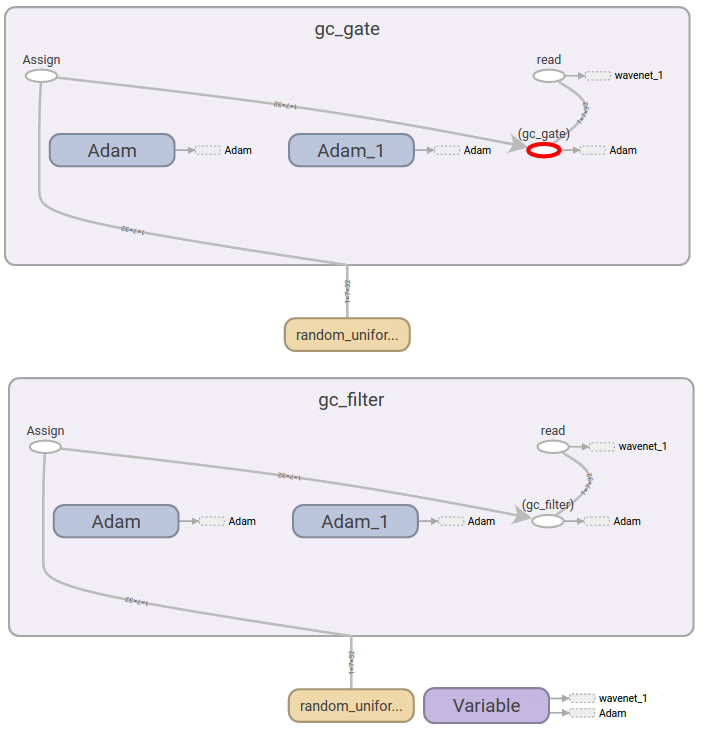
\includegraphics[scale=1]{img/gc}
  \caption{Глобальные условия в архитектуре}
  \label{fig:gc}
\end{figure}


% \subsection{Локальные условия}
В архитектуре это выглядит почти симметрично для локальных и глобальных условий с точностью до размерности тензоров. Мы должны добавить пару (\verb|gc_filter|, \verb|gc_gate|) и (\verb|lc_filter|, \verb|lc_gate|) для глобальных и локальных условий соответственно, чтобы потом передать результат свёртки с ними на update gate. Для глобальных условий на фиксированном слое это изображено на рисунке \ref{fig:gc}.


    
\newpage    

\subsubsection{Обработка условий}

Давайте ещё  раз вспомним, по каким каналам данные поступают в WaveNet:

\begin{itemize}
    \item Сырые данные.
    \begin{itemize}
        \item Временной ряд, цифровое представление голоса по времени.
    \end{itemize}
    \item Локальное условие .
    \begin{itemize}
        \item Временной ряд, той же длины что и данные. Качество, изменяющееся по времени.
    \end{itemize}
    \item Глобальное условие.
    \begin{itemize}
        \item Качество говорящего, не зависящее от времени. Не меняет своего значения в процессе обучения/генерации.
    \end{itemize}
\end{itemize}


Прежде чем быть переданными на вход нейросети данные должны имть чётко структурированное векторизованное представление. Однако недостаточно просто закодировать данные. На самом деле мы провели преобразование данных в векторный вид ещё не стадии извлечения признаков, что порождает вопрос, почему бы и не передавать это представление в качестве условий.
На самом деле это было бы невозможно даже с точки зрения архитектуры. Ещё во вводной части мы упоминали, что условия должны быть выровнены вдоль данных, то есть иметь ту же длину. Если говорить о звуке как о временном ряде, то временной ряд условий должен иметь ту же длину, что и голос, однако на ширину архитектура ограничений не налагает.

\subsubsection{Глобальные условия}

В первую очередь опишем проблему построения глобальных условий, поскольку она решается проще. С точки зрения временного ряда глобальное условие это значение, константное во все моменты времени. Поэтому для глобальных условий достаточно продублировать значение признака необходимое количество раз.

\subsubsection{Локальные условия}

С локальными условиями дело обстоит сложнее, поскольку разные признаки могут иметь разную длину. Каждый признак требует индивидуального ad hoc решения. Это связано с тем, что локальное условие должно не только иметь требуемую архитектурой длину, но и быть актуальным в момент аудио, которому сопоставлено.

Разберём на примере одного признака.
Наиболее сложный случай возникает когда признаки извлекаются не из звукового отрезка, а из соответствующего ему текстового файла. Мало того что у нас текст не выровнен по звуку, так ещё и из этого текста мы извлекаем признаки, получая двойную погрешность в выравнивании.

В качестве примера опишем достаточно интуитивный пример локального условия, основывающийся на тексте.
На рисунке \ref{fig:arch_low} изображено, какой путь проходит текст, прежде чем попасть в \verb|dilated_stack|.

% \begin{centering}
$$
\verb|one_hot_1| \rightarrow \verb|ExpandDimention| \rightarrow \verb|Resize| \rightarrow \verb|Squeeze|.
$$
% \end{centering}
% $$
% \verb|one_hot_1| \rightarrow \verb|ExpandDimention|
% $$

В качестве кодирования будем хэшировать каждый символ, после чего растягивать полученный ряд вдоль звука. 
Интуитивный эквивалент такого преобразования будет выглядеть так:

$$
\verb|'The car'| \rightarrow \verb|'TTTTTTThhhhhhheeeeee      cccccaaaarrrr'|.
$$

\begin{figure}[ht!]
  \centering
  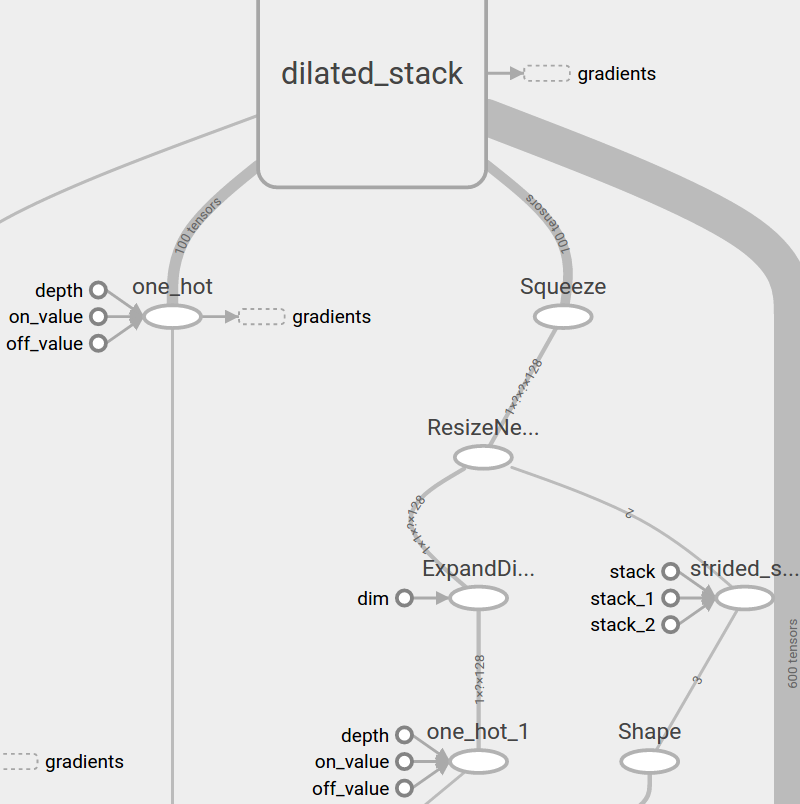
\includegraphics[scale=1]{img/arch}
  \caption{Обработка локальных текстовых условий}
  \label{fig:arch_low}
\end{figure}


% \subsubsection{Репозиторий}
% Наша реализация WaveNet доступна по ссылке \cite{github:repo}.

\newpage
\pagebreak

\subfile{sections/feature_engineering}

\end{document}

